%latex report

\documentclass[a4paper,11pt]{article}
\usepackage{times}
\usepackage{graphicx}
%\usepackage{amsmath}
\usepackage{natbib}
\usepackage[top=2.54cm, bottom=2.54cm, right=1.27cm, left=1.27cm]{geometry}
\begin{document}


\title{Physics Behind the Simulation: A CS296 Group 31 Report.}

\author{Sanchit Garg\\ 110050035\\	\texttt{sanchitgarg@cse.iitb.ac.in} \and
		Ravi Kumar Roshan\\ 110050033\\ \texttt{sraviroshan@cse.iitb.ac.in}
		}

\date{10 April, 2013}

\maketitle


\section{Introduction}
A Rube Goldberg machine, contraption, invention, device, or apparatus is a deliberately over-engineered or overdone machine that performs a very simple task in a very complex fashion, usually including a chain reaction. The expression is named after American cartoonist and inventor Rube Goldberg (1883–1970). %////Wikipedia

This is a small Project Report about the simulation and contraption using C++ Simulator engine Box2D under the CS296 Lab Course.

Here we first describe the design of the simulation followed by its timing and Profiling issues.

\section{Design}
First we start with implemented design. Design is very simple. Implemented and original design are almost same. We then describe some minor changes we have done in original design.
\subsection{Implemented Design}	

\begin{center}
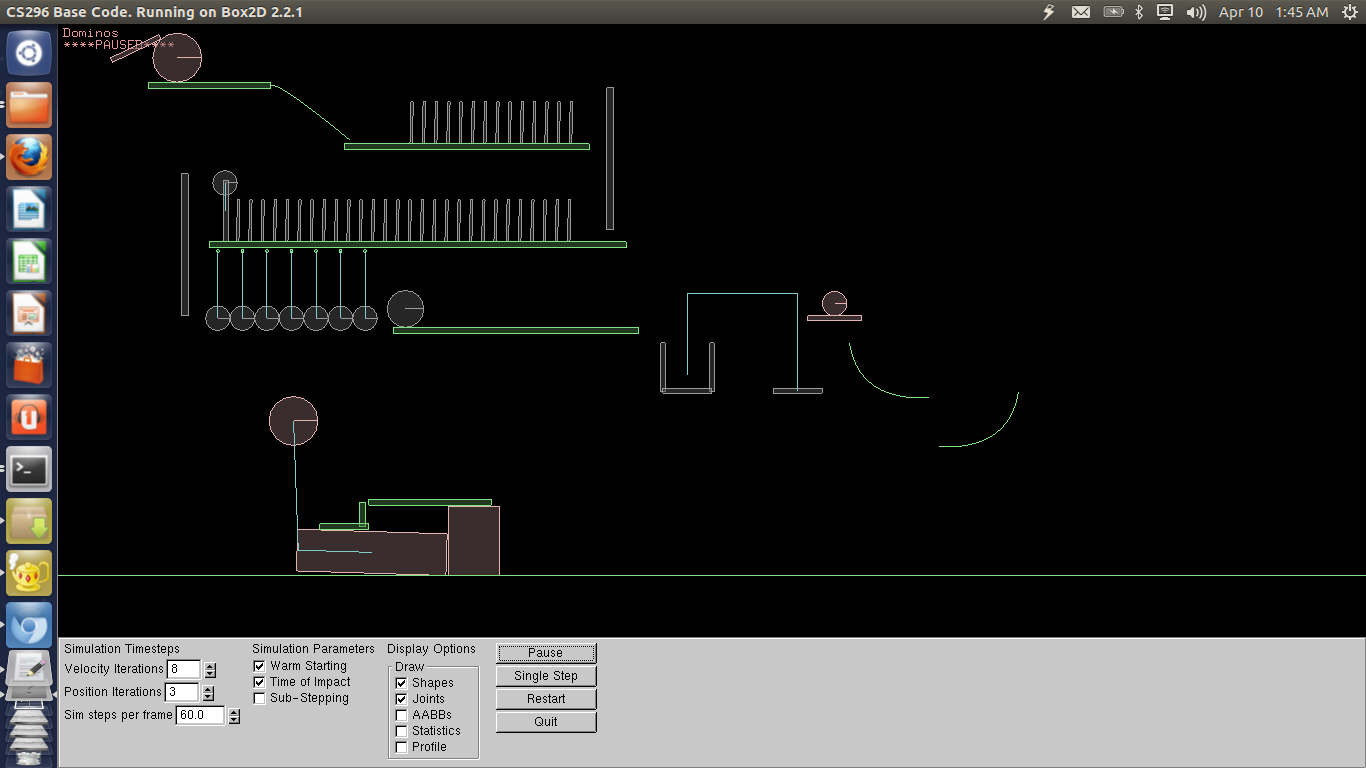
\includegraphics[scale=0.3]{./doc/photo1.png}
\begin{center}
Fig.1
\end{center}
\end{center}

First a Motored plank. It starts revolving and strikes a ball resting on a platform. 
This ball rolls down from a slope and hits the train of Dominos standing on horizontal Platform. Dominos start falling. There is a rotating shaft near the end of this domino train. It gets hit by the dominos. This shaft while rotating hits another train of Dominos standing on another horizontal platform just below the first one. On the end of this domino train there is another rotating shaft which do the same purpose that as of the previous one. This rotates on hit by dominos. On the way of its rotaion Newton's Cradle is kept. Shaft hits the Newton's Cradle. Near the end of the Cradle a ball is kept. This  ball get struck by the cradle and rolls horizontally and finally enters in pully system. There is a Bucket(open box) into which the ball falls. When this ball falls, the bucket becomes heavier and starting coming dowm and as a result the other side of pulley which is connected by a horizontal plank, starts moving up and make rotates the another horizontal platform. There is a ball resting on this platform which falls down due to movement of platform. This ball follows a zig-zag path on two curves and falls on ground and moves towards a piston. Finally the ball hits the piston. On the mouth of piston there is a block attached with a balloon. This balloon is basically a ball whose gravity is reversed. Ball coming towards the piston hits and balloon moves up along with block.

\subsection{Original Design}
There are 3 changes apart from body's structure :
\begin{center}
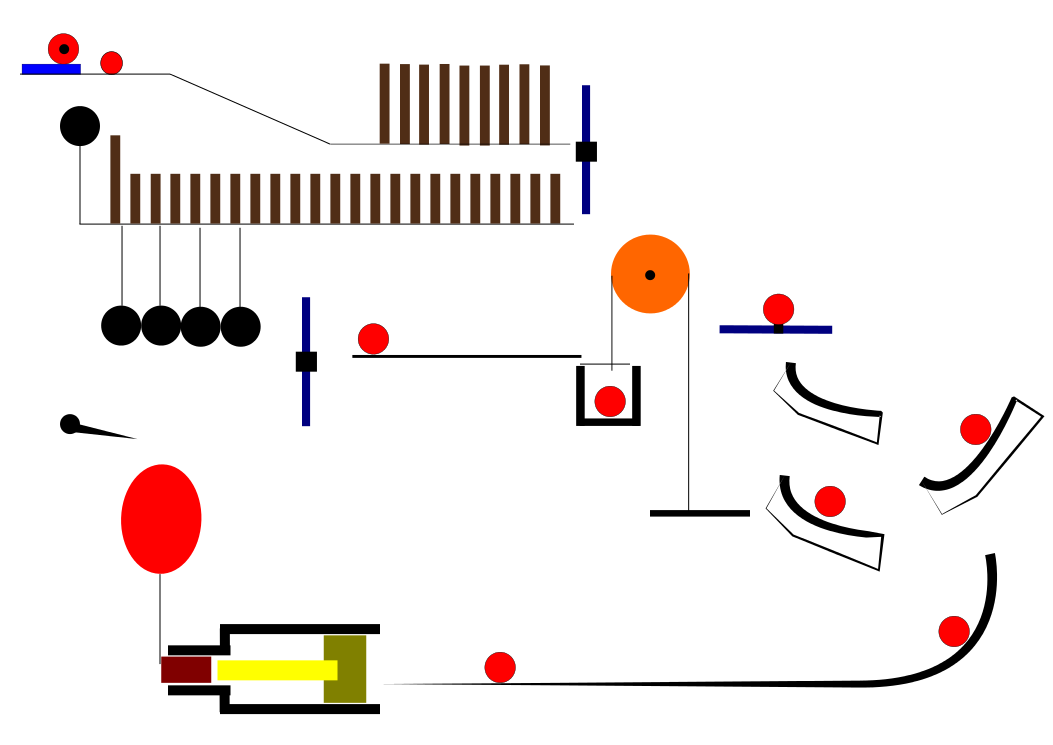
\includegraphics[scale=0.3]{./doc/idea.png}
\begin{center}
Fig.2
\end{center}
\end{center}

\begin{itemize}
\item {Motored Plank}
\begin{description} Instead of motored plank We thought of a revolving ball which is in contact with a plank. As ball rotates plank moves and hit a ball and continue.
\end{description}

\item {Second Revolving Shaft}
\begin{description} Instead of second revovling shaft We planned that at the end of the second dominos train there is a inverted pendulum standing and on hit it moves down and starts the motion of Newton's Cradle.
\end{description}

\item{Bursting of Balloon}
\begin{description} We thought that as the balloon rise it would come into the contact of a pointed thing and will burst.
\end{description}
\end{itemize}

\subsection{Interesting Features}
\begin{itemize}
\item {Newton's Cradle}
\begin{description} Newtons Cradle may look like interesting but in simulation the exact effect of it has not achieved i.e only end balls move.
\end{description}

\item {Rising Balloon}
\begin{description} Rising Balloon (acieved by reversing its gravity) may look like interesting.
\end{description}
\end{itemize}


\section{Profiling}
A profiler is used to identify what are the parts of your code are taking the maximum time. This helps in identifying parts of your code that can be optimized. Here below is the profiling done first with optimization i.e with release mode on and second with debugging mode on. For profiling we have used perf tool.

\subsection{Observations}
Analysis has beem done on the iteration no. 200, 1000 and 5000.
\begin{itemize}
\item{For Iteration no. 200}
\begin{description} In debug mode maximum time is taken by "b2ContactSolver::SolveVelocityConstraints()" approx. 19.55\% while in release mode maximum time is taken by "b2World::Step(float, int, int)" approx. 11.13\% but next is "b2ContactSolver::SolveVelocityConstraints()" approx. 9.15\%.
\end{description}

\item{For Iteration no. 1000}
\begin{description} In debug mode maximum time is taken by "b2ContactSolver::SolveVelocityConstraints()" approx. 9.55\% while in release mode maximum time is taken by "b2EdgeSeparation(b2PolygonShape const*, b2Transform const\&, int, b2PolygonShape const*)" approx. 20.13\% but next is "b2ContactSolver::SolveVelocityConstraints()" approx. 15\%.
\end{description}

\item{For Iteration no. 5000}
\begin{description} In both mode maximum time is taken by "b2ContactSolver::SolveVelocityConstraints()" approx. 6.33\% in debug mode and 18.20\% in release mode.
\end{description}

\end{itemize}

\subsection{Call Graphs}
The call graph shows how much time was spent in each function and it’s children. Here is the call grpahs for both release and debug mode for iteration no. 200. We can see clearly the complexity of the running the simulation in both the cases.

\begin{center}
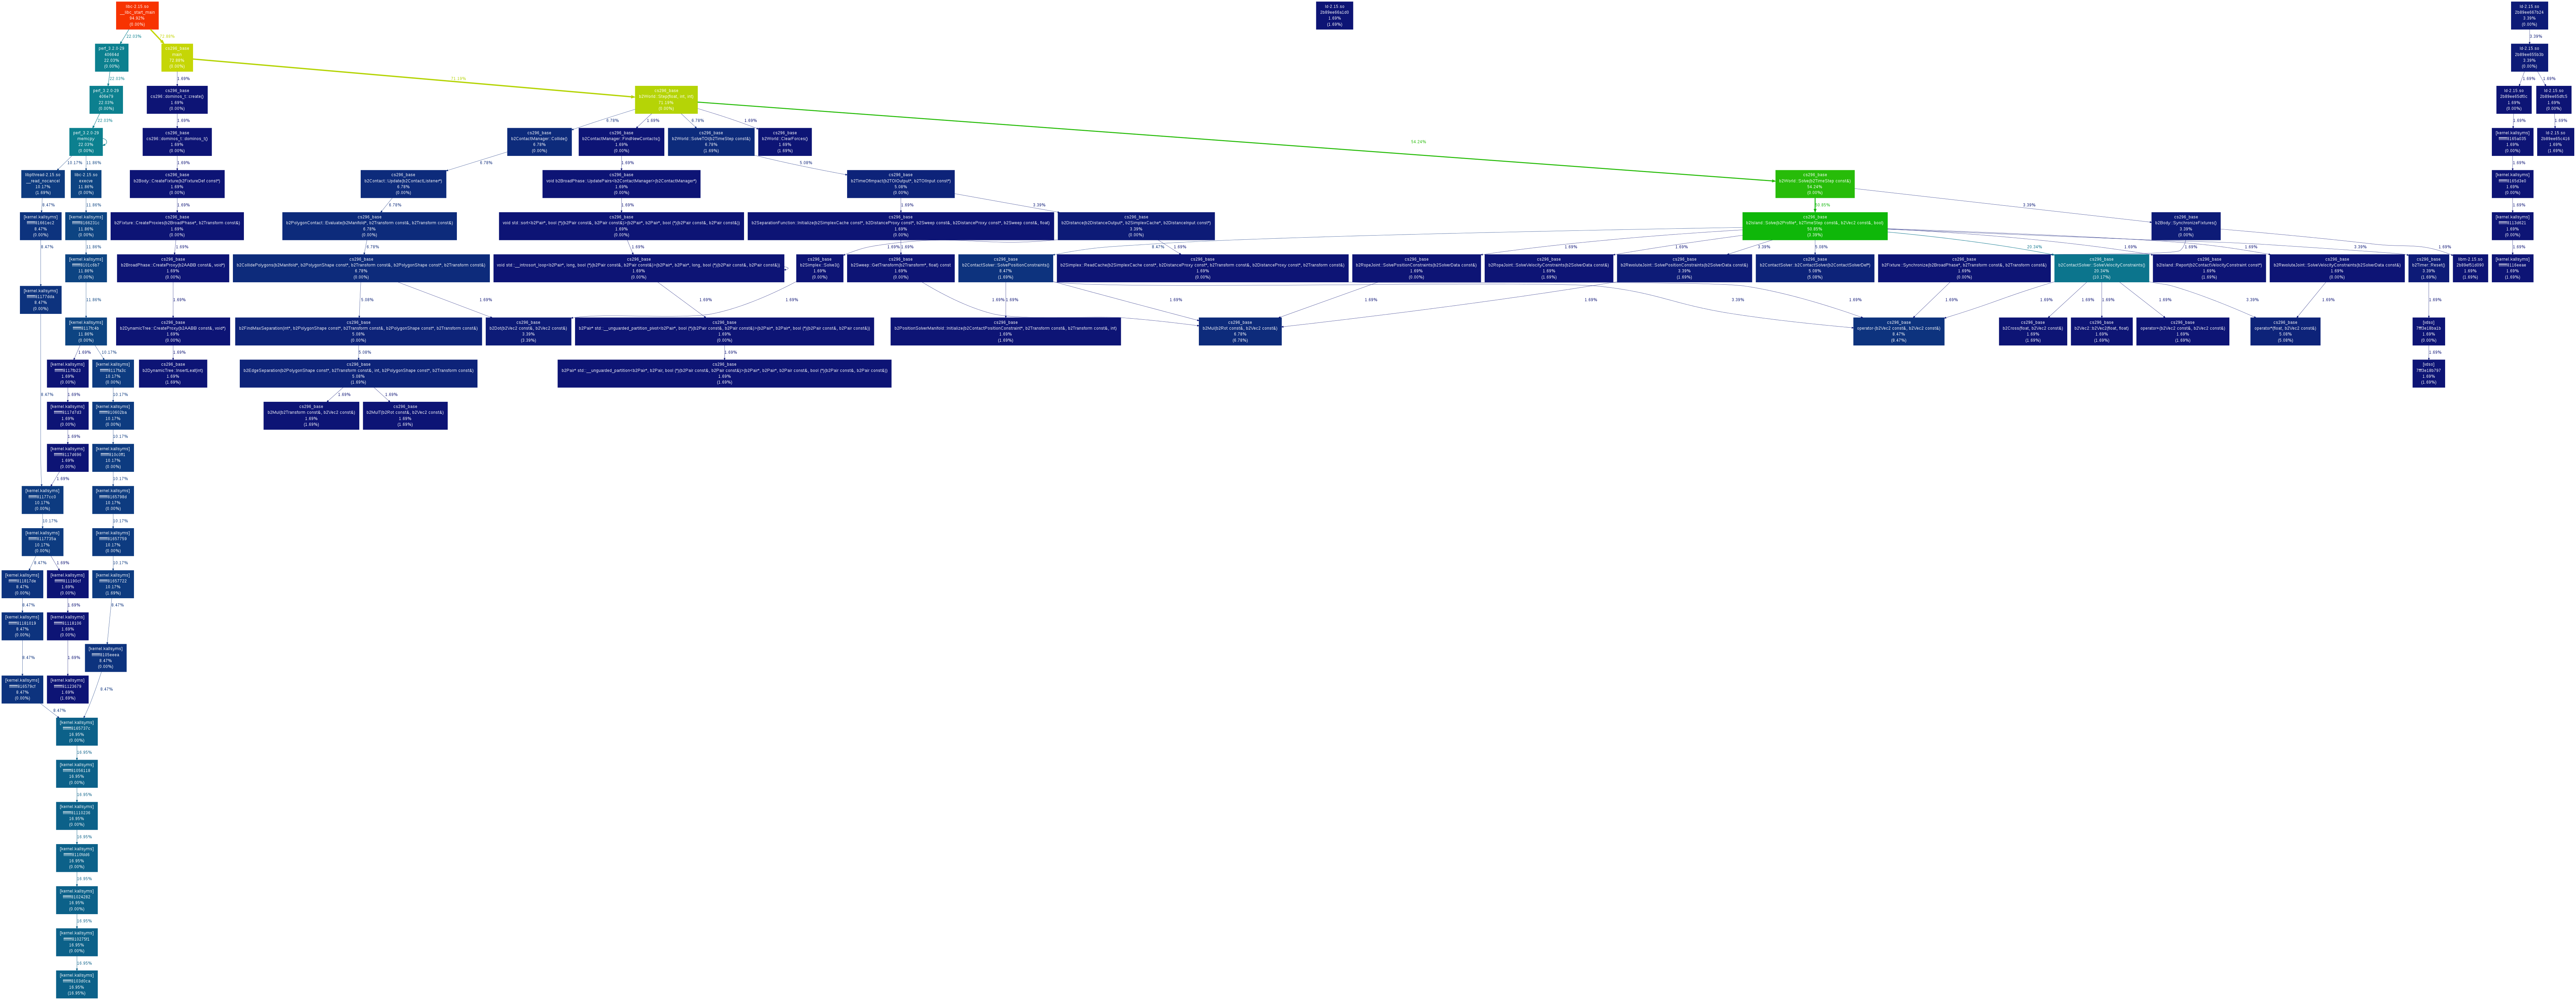
\includegraphics[scale=0.1]{./doc/deb_output200.png}
\begin{center}
Fig.3 Call Graph for Debug Mode:Itr value 200
\end{center}
\end{center}

\begin{center}
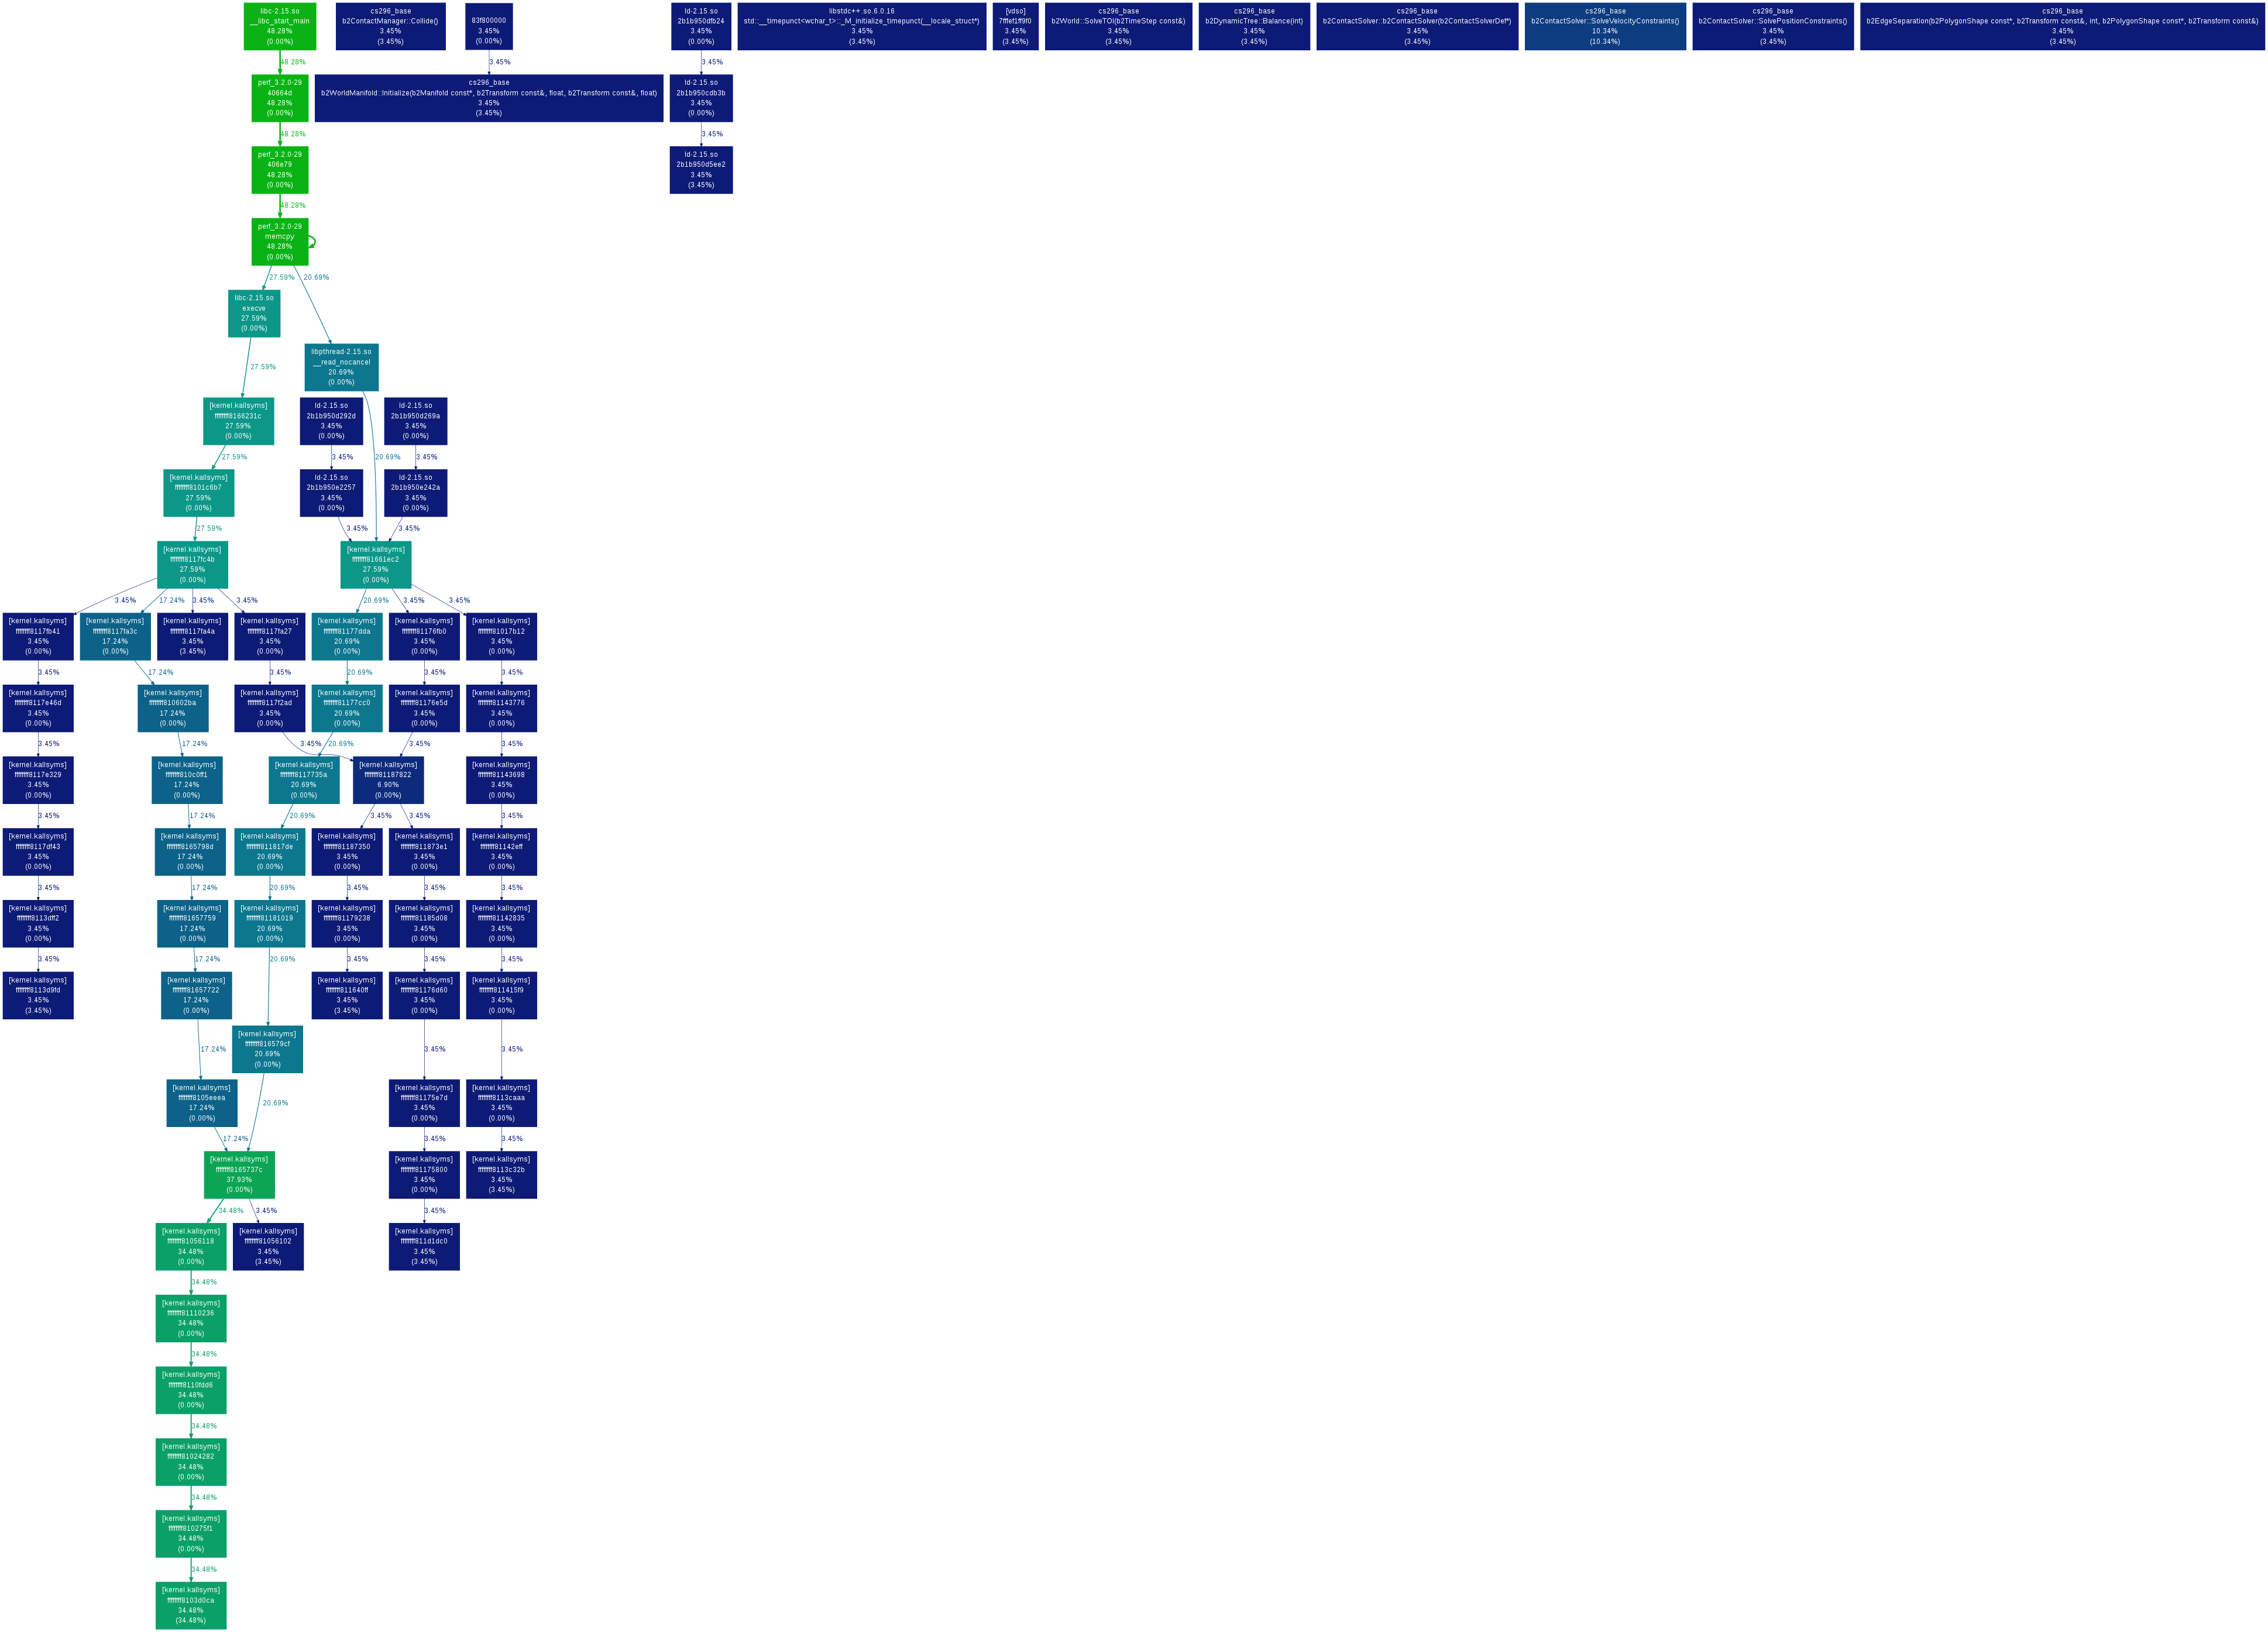
\includegraphics[scale=0.1]{./doc/rel_output200.png}
\begin{center}
Fig.3 Call Graph for Release Mode:Itr value 200
\end{center}
\end{center}

\subsection{Conclusion}
\begin{itemize}
\item{We can see that number of functions calls for constructors are reduced drastically in the release part as compared to debug part and hence indicates that optimization flags work on constructors.}

\item{Here is a consistent observation. Most of the time is taken by method "b2ContactSolver::SolveVelocityConstraints()". Hence there is a possiblity of implementation optimization of this function in Box2D Library.}
\section{Conclusion}
Thus in the report we have analyzed and timed the code under different conditions and summerized the results.
\end{itemize}
\end{document}
